\documentclass[12pt, a4paper]{article}
\usepackage{amsfonts, amssymb,amsmath}
\usepackage{graphicx}
\usepackage{dsfont}
\usepackage[margin=1.0in]{geometry}
\linespread{1} 


\begin{document}

\begin{titlepage}
   \begin{center}
       \vspace*{0.5cm}

       \LARGE{\textbf{Assignment 1}}

       \vspace{1cm}
        \Large{Advanced Classical Mechanics}
            
       \vspace{1cm}
		\small{Gavin Kerr (B00801584)} \\
		\vfill
		
\includegraphics[scale=0.65]{dal_logo2.png}
       \vfill
           \large{PHYC 3590}
            
       \vspace{0.8cm}
     
            
       Physics and Atmospheric Science\\
       Dalhousie University\\
       2022-01-16
            
   \end{center}
\end{titlepage}



\section*{Question 1.16}
\subsection*{(a)}
Show that $|r| = \sqrt{r\cdot r}$. Firstly, let $r = x\hat{x} + y \hat{y} + z \hat{z}$.
\begin{align*}
r =& x\hat{x} + y \hat{y} + z \hat{z}
\\
r\cdot r =& (x\hat{x} + y \hat{y} + z \hat{z})(x\hat{x} + y \hat{y} + z \hat{z})
\\
r\cdot r =& x^2 + y^2 + z^2 = r^2
\\
r\cdot r =& r^2
\\
\sqrt{r\cdot r} =& \sqrt{r^2}
\\
\sqrt{r\cdot r} =& |r|
\\
&\text{QED}
\end{align*}
\subsection*{(b)}
Prove that $r\cdot s$, as defined by (1.7), is the same for any choice of orthogonal axes. 
\begin{align*}
|r|
\end{align*}





\section*{Problem 1.26}
\subsection*{(a)}
For $S$ we have $x=0, y=v_1t$, where $v_1$ is the speed at which the man kicks the puck.
\subsection*{(b)}
For $S'$ relative to $S$ we have $x=v_2t, y=0$, where $v_2$ is the speed of the second observer relative to the first observer ($S$). In the $S'$ frame, the path of the puck would be $x'= x_1-v_2t, y'=y_1 +v_1t$. $(x_1, y_1)$ is the distance between observer 1 \& 2. 
\subsection*{(c)}
For $S''$ relative to $S$, we have $x=\tfrac{1}{2}at^2, y=0$, where $a$ is the acceleration of the third observer. In the $S''$ frame, the puck follows the path $x=x_2-\tfrac{1}{2}at^2 y=y_2+v_1t$. $(x_2,y_2)$ is the distance between the first \& third observer.\\
\\
The $S$ and $S'$ are inertial reference frames. $S''$ is not an inertial reference frame because it is accelerating.





\section*{Problem 1.31}
I think this question needs more. 
\begin{align*}
P_1 + P_2 =& c
\\
\frac{dP_1}{dt} + \frac{dP_2}{dt} =& \frac{dc}{dt}
\\
F_1 + F_2 =& 0
\\
F_1 =& - F_2
\\
\text{QED}
\end{align*}





\pagebreak
\section*{Problem 1.39}
\begin{figure}[h]
  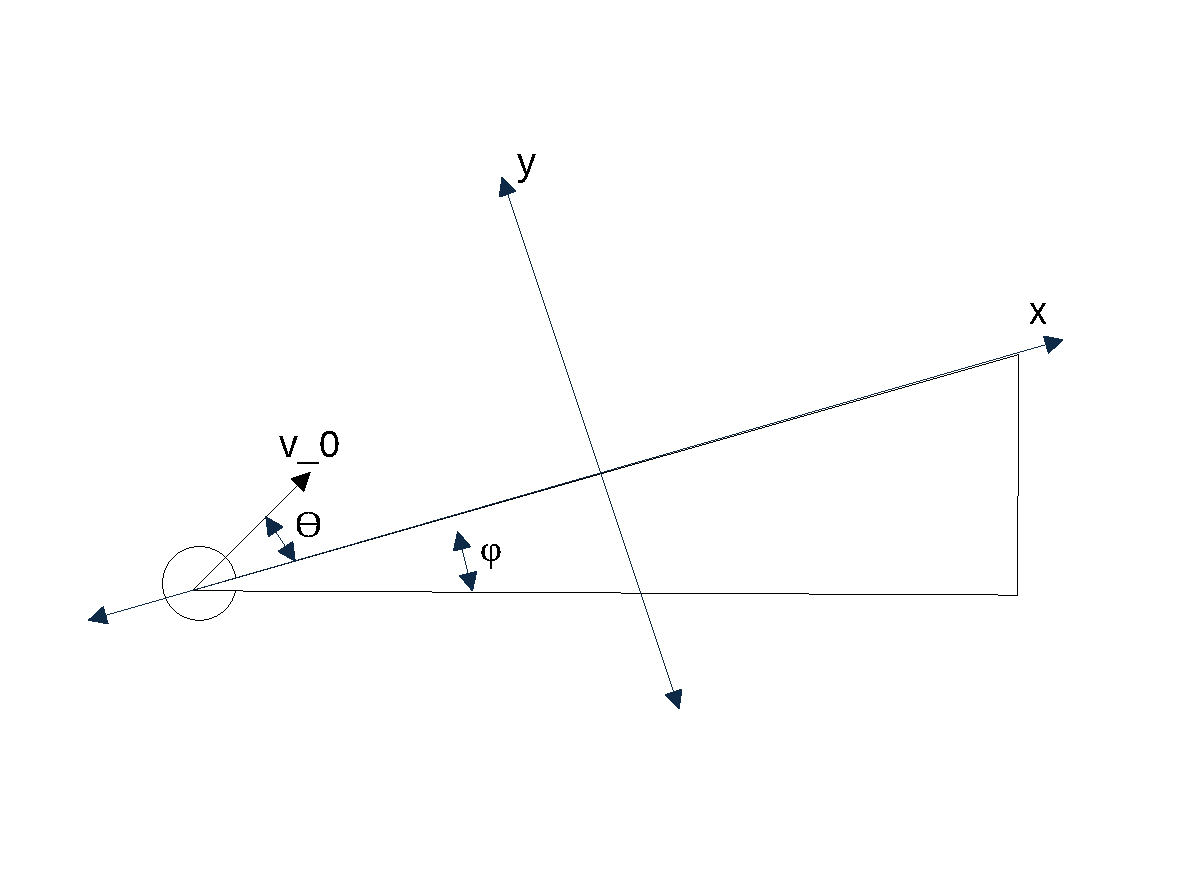
\includegraphics[width=4in]{fig_1.pdf}
  \caption{Diagram}
  \label{fig_1}
\end{figure}
For the initial conditions, we have $\vec{v_0}$. Also there is only one force acting on the object $\vec{F_g}$ which means that $\vec{g}$ is the acceleration. Solving for the equations of motion, we have
\begin{align*}
\vec{g} =& -g(\sin\phi \hat{x}+\cos\phi \hat{y})
\\
\vec{v} =& \int \vec{g} \,dt + \vec{v_0}
\\
\vec{v_0} =& v_0(\cos\theta\hat{x}+\sin\theta\hat{y})
\\
\vec{v} =& -g(\sin\phi \hat{x}+\cos\phi \hat{y})t + |v_0|(\cos\theta\hat{x}+\sin\theta\hat{y})
\\
\vec{r} =& \int \vec{v} \,dt
\\
\vec{r} =& \int -g(\sin\phi \hat{x}+\cos\phi \hat{y})t + |v_0|(\cos\theta\hat{x}+\sin\theta\hat{y}) \, dt
\\
\vec{r} =& -g(\sin\phi \hat{x}+\cos\phi \hat{y})\frac{t^2}{2} + |v_0|(\cos\theta\hat{x}+\sin\theta\hat{y})t
\\
x =& v_0\cos\theta \,t - \tfrac{1}{2}g\sin\phi \,t^2
\\
y =& v_0\sin\theta \,t - \tfrac{1}{2}g\cos\phi \,t^2
\end{align*}
Next we want to find out for how long, the ball is in the air. To do this, we need to find the difference of the two roots of the equation for $y$. The first root is trivially $t_1=0$. For the second root, $t_2 = \Delta t$, we have
\begin{align*}
0 =& |v_0|\sin\theta \,t - \tfrac{1}{2}|g|\cos\phi \,t^2
\\
0 =& |v_0|\sin\theta  - \tfrac{1}{2}|g|\cos\phi \,t
\\
\tfrac{1}{2}g\cos\phi \,t =& |v_0|\sin\theta
\\
t_2 =& \dfrac{2|v_0|\sin\theta}{g\cos\phi}
\end{align*}
This means the the ball touches the ramp at $t = \dfrac{2|v_0|\sin\theta}{g\cos\phi}$. Subbing this into the equation for $x$ to find the final position gives us
\begin{align*}
x =& |v_0|\cos\theta \left(\dfrac{2v_0\sin\theta}{g\cos\phi}\right) - \tfrac{1}{2}g\sin\phi \left(\dfrac{2v_0\sin\theta}{g\cos\phi}\right)^2
\\
x =&  \left(\dfrac{2v_0^2\sin\theta\cos\theta}{g\cos\phi}\right) -  \left(\dfrac{2v_0^2\sin^2\theta\sin\phi}{g\cos^2\phi}\right)
\\
x =&  \frac{2v_0^2}{g}\left(\dfrac{\sin\theta\cos\theta}{\cos\phi} -  \dfrac{\sin^2\theta\sin\phi}{\cos^2\phi}\right)
\\
x =&  \frac{2v_0^2}{g}\left(
\dfrac{\sin\theta\cos\theta\cos\phi}{\cos^2\phi} -  
\dfrac{\sin^2\theta\sin\phi}{\cos^2\phi}
\right)
\\
x =&  \frac{2v_0^2}{g}\left(
\dfrac{\sin\theta\cos\theta\cos\phi - \sin^2\theta\sin\phi}{\cos^2\phi}
\right)
\\
x =&  \frac{2v_0^2}{g}\left(
\dfrac{\sin\theta(\cos\theta\cos\phi - \sin\theta\sin\phi)}{\cos^2\phi}
\right)
\\
x =&  \frac{2v_0^2}{g}\left(
\dfrac{\sin\theta\cos(\theta+\phi)}{\cos^2\phi}
\right)
\\
x =& \boxed{R = \dfrac{2v_0^2\sin\theta\cos(\theta+\phi)}{g\cos^2\phi}}
\\
&\text{QED}
\end{align*}
To solve for $R_{max}$ we need to find a local max for $R$ as a function of $\theta$, where $\tfrac{dR}{d\theta}=0$.
\begin{align*}
\frac{dR}{d\theta} =& \frac{d}{d\theta}\dfrac{2v_0^2\sin\theta\cos(\theta+\phi)}{g\cos^2\phi}
\\
\frac{dR}{d\theta} =& \dfrac{2v_0^2}{g\cos^2\phi}\frac{d}{d\theta}\left(\sin\theta\cos(\theta+\phi)\right)
\\
\frac{dR}{d\theta} =& \dfrac{2v_0^2}{g\cos^2\phi}\left(
\cos\theta\cos(\theta+\phi) -
\sin\theta\sin(\theta+\phi)
\right)
\\
\frac{dR}{d\theta} =& \dfrac{2v_0^2}{g\cos^2\phi}\cos(2\theta+\phi)
\\
0 =& \dfrac{2v_0^2}{g\cos^2\phi}\cos(2\theta+\phi)
\\
\pi/2 =& 2\theta+\phi
\\
\pi/2 - \phi =& 2\theta
\\
\theta_{max} =& \frac{\pi-2\phi}{4}
\end{align*}
Next, we just sub $\theta$ into the equation for $R$ to find the maximum distance.
\begin{align*}
R_{max} =& \dfrac{2v_0^2\sin\theta\cos(\frac{\pi-2\phi}{4}+\phi)}{g\cos^2\phi}
\\
R_{max} =& \dfrac{2v_0^2\sin\theta\cos(\frac{\pi-2\phi+4\phi}{4})}{g\cos^2\phi}
\\
R_{max} =& \dfrac{2v_0^2\sin\theta\cos(\frac{\pi+2\phi}{4})}{g\cos^2\phi}
\\
R_{max} =& \dfrac{2v_0^2\sin\theta\cos(
\frac{\pi}{4} + 
\frac{\phi}{2}
)}{g\cos^2\phi}
\\
R_{max} =& \dfrac{2v_0^2\sin\theta
[\cos(\frac{\pi}{4})
\cos(\frac{\phi}{2}) -
\sin(\frac{\pi}{4})
\sin(\frac{\phi}{2})]
}{g\cos^2\phi}
\\
R_{max} =& \dfrac{2v_0^2\sin\theta
[\frac{\sqrt{2}}{2}
\cos(\frac{\phi}{2}) -
\frac{\sqrt{2}}{2}
\sin(\frac{\phi}{2})]
}{g\cos^2\phi}
\\
R_{max} =& \dfrac{\sqrt{2}v_0^2\sin(\frac{\pi-2\phi}{4})
[\cos(\frac{\phi}{2}) - \sin(\frac{\phi}{2})]
}{g\cos^2\phi}
\\
R_{max} =& \dfrac{\sqrt{2}v_0^2
\sin(\pi/4-\phi/2)
[\cos(\frac{\phi}{2}) - \sin(\frac{\phi}{2})]
}{g\cos^2\phi}
\\
R_{max} =& \dfrac{\sqrt{2}v_0^2
[\sin(\pi/4)
\cos(\phi/2) -
\cos(\pi/4)
\sin(\phi/2)]
[\cos(\frac{\phi}{2}) - \sin(\frac{\phi}{2})]
}{g\cos^2\phi}
\\
R_{max} =& \dfrac{\sqrt{2}v_0^2
[\sqrt{2}/2
\cos(\phi/2) -
\sqrt{2}/2
\sin(\phi/2)]
[\cos(\frac{\phi}{2}) - \sin(\frac{\phi}{2})]
}{g\cos^2\phi}
\\
R_{max} =& \dfrac{v_0^2
[\cos(\frac{\phi}{2}) - \sin(\frac{\phi}{2})]
[\cos(\frac{\phi}{2}) - \sin(\frac{\phi}{2})]
}{g\cos^2\phi}
\\
R_{max} =& \dfrac{v_0^2
[\cos^2(\frac{\phi}{2}) - 2\sin(\frac{\phi}{2})\cos(\frac{\phi}{2})+
\sin^2(\frac{\phi}{2})]
}{g\cos^2\phi}
\\
R_{max} =& \dfrac{v_0^2
[1 - 2\sin(\frac{\phi}{2})\cos(\frac{\phi}{2})]
}{g\cos^2\phi}
\\
R_{max} =& \dfrac{v_0^2
[1 - \sin\phi]
}{g\cos^2\phi}
\\
\end{align*}
I think this should be correct but I don't know which trig identity so simplify the expression so what is given in the question, $R_{max} = \frac{v_0^2}{g[1+\sin\phi]}$. 




\pagebreak
\section*{Problem 1.46}
\begin{align*}
...
\end{align*}






















\end{document}
